% \subsection{Value functions in belief wealth space}

As described in~\autoref{sec:methods} augmented state space encodes the wealth and the belief of the agent. Note that time can be derived from wealth, in our setting exactly by $\text{time} = \text{wealth} / \text{observation cost}$.

First, we look at value functions found by using different utility functions in~\autoref{fig:val-func}.
Value functions found by exponential utility show that the induced behaviour is independent of time and risk is only modeled by the belief threshold the agent decides to sell at. This threshold is set by the $\lambda$ parameter, which is displayed on above the plot.

On the other hand, the sinh utility function is able to model time dependent behaviour, e.g. selling at a fixed time step. We have parametrized sinh by the scaling and shifting of its input:

\begin{align*}
    U_\text{sinh}(v) := \frac{e^v' - e^{-v'}}{2} \text{, where } v' = \text{scale}\cdot(v+\text{shift})
\end{align*}

Scale and shift parameters are displayed above each plot.

Lastly, we present the dynamic utility function where $\lambda_i$ is selected from a logarithmically spaced sequence. The sequence range is displayed above each plot.

% TODO: use sinh with better parametrization

\begin{figure}[H]
    \centering
    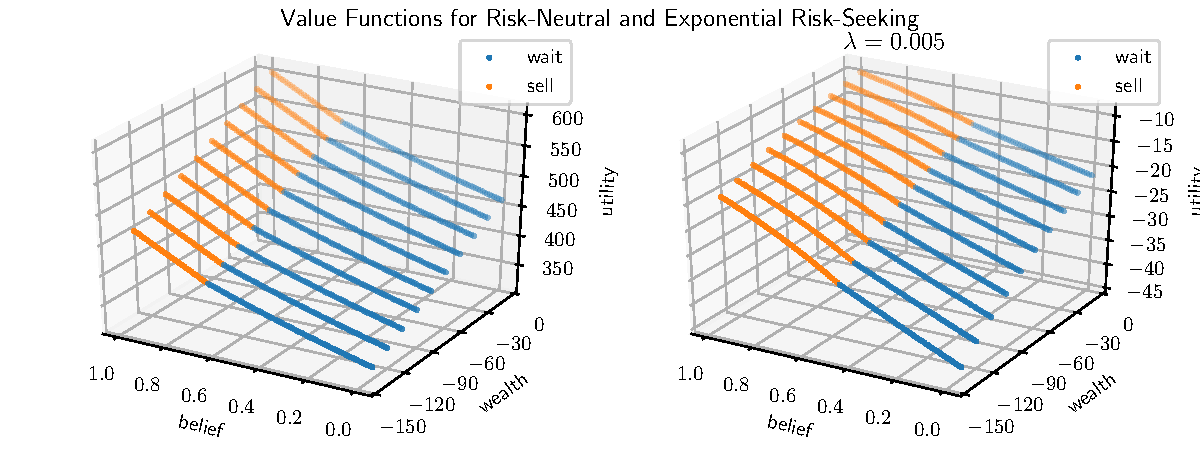
\includegraphics[width=0.98\linewidth]{img/exp_policy.pdf}\\
    \vspace{1cm}
    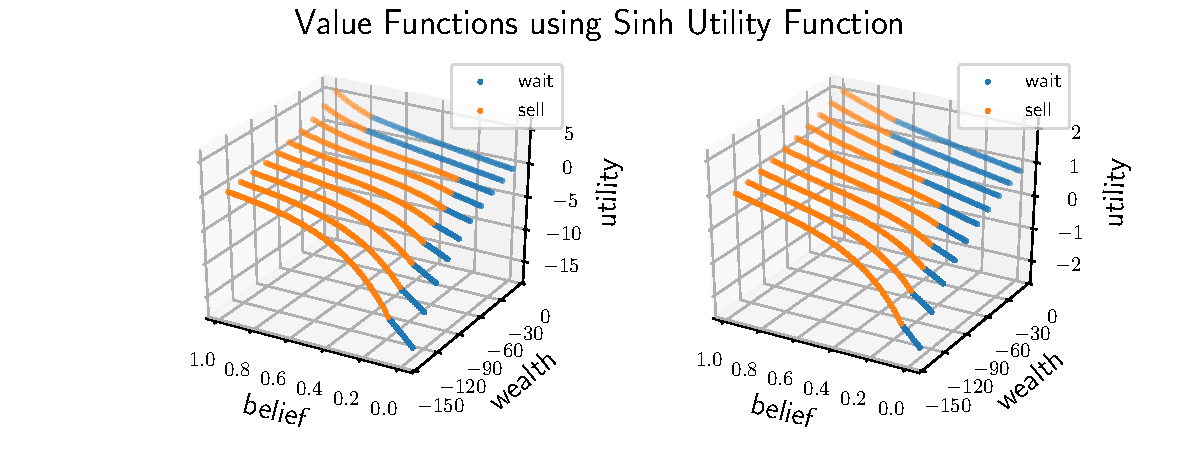
\includegraphics[width=0.98\linewidth]{img/sinh_policy.pdf}\\
    \vspace{1cm}
    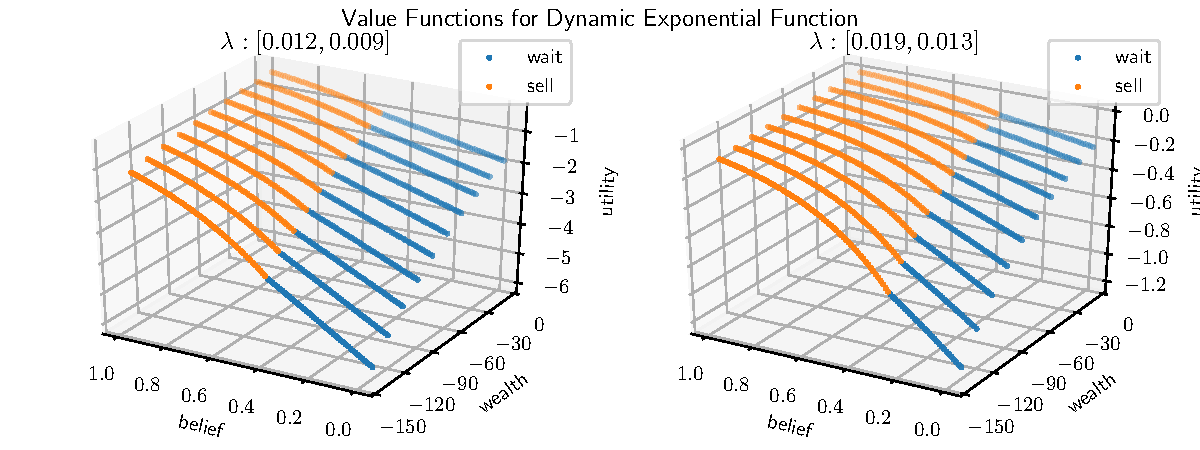
\includegraphics[width=0.98\linewidth]{img/dyn_policy.pdf}
    \caption{Value functions exhibiting different risk-behaviors; from top left: risk neutral agent (utility function is the identity function), risk-seeking agent with exponential utility function, two fixed time agents with different time thresholds, two agents with dynamic exponential utility function.}\label{fig:val-func}
\end{figure}



\subsection{From human behavior to utility functions}


\normalsize
\textbf{The original problem:}
\begin{itemize}
\item[①] Choose utility function with risk parameter.
\item[②] Perform value iteration.
\item[③] Derive policy.
\end{itemize}

\textbf{The inverse problem:}
\begin{itemize}
\item[①] Observe behavior.
\item[②] Estimate policy.
\item[③] Derive utility function and risk parameters.
\end{itemize}

The original problem is easy to solve, unfortunately for the inverse problem no solution is known. 

$\rightarrow$ Perform grid-search and choose optimal utility function.

\begin{figure}
    \centering
    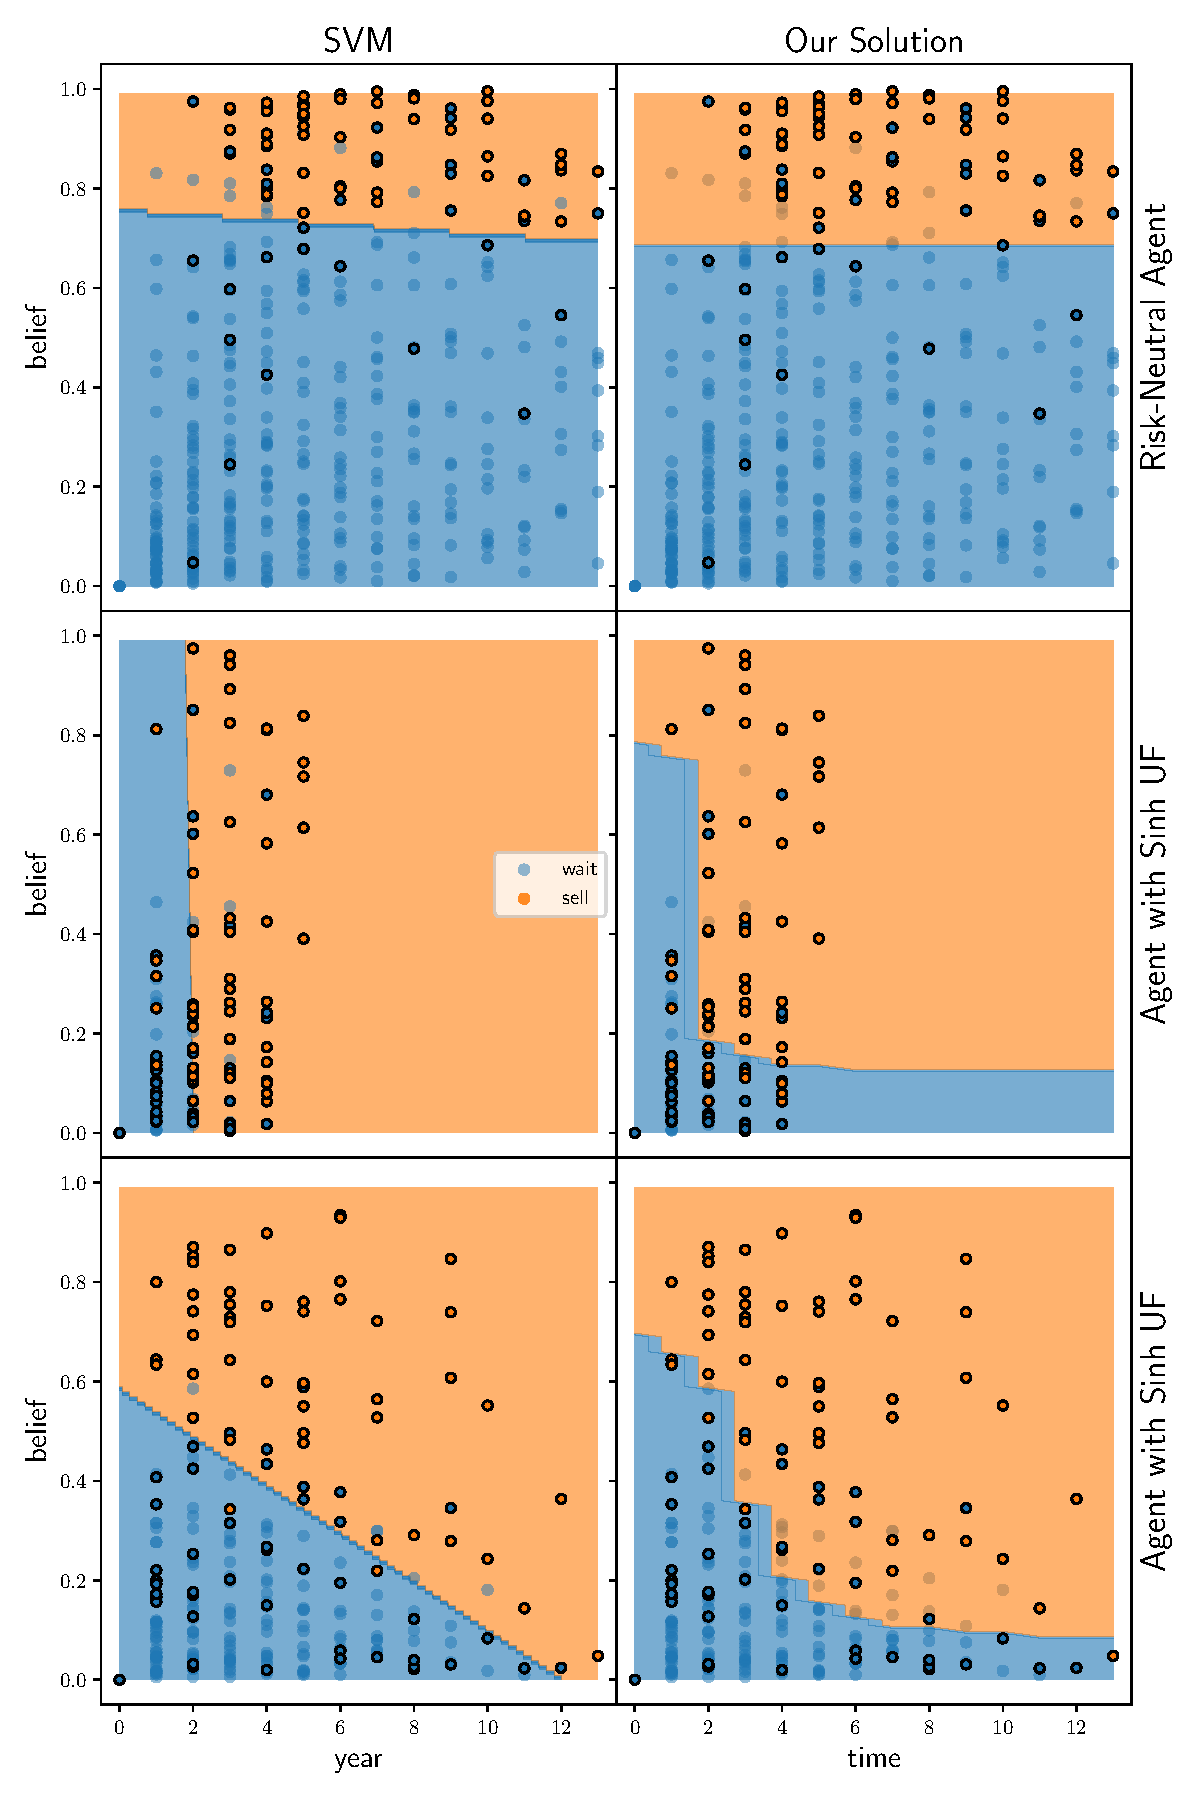
\includegraphics[width=0.8\linewidth]{img/fit}
    \caption{Examples from three human behaviors distinctly observed and replicated with RL agents. Behaviours by row: 1) Constant belief threshold, modelled by exponential utility, 2) Fixed time threshold, modelled by sinh utility, 3) Mixed strategy, modelled by dynamic exponential utility. Left column shows empirical optimal split of data using cross validation and linear kernel support vector machines, right column shows optimal policy found via gridsearch.}
    \label{fig:svm_vs_value}
\end{figure}

\begin{figure}
    \centering
    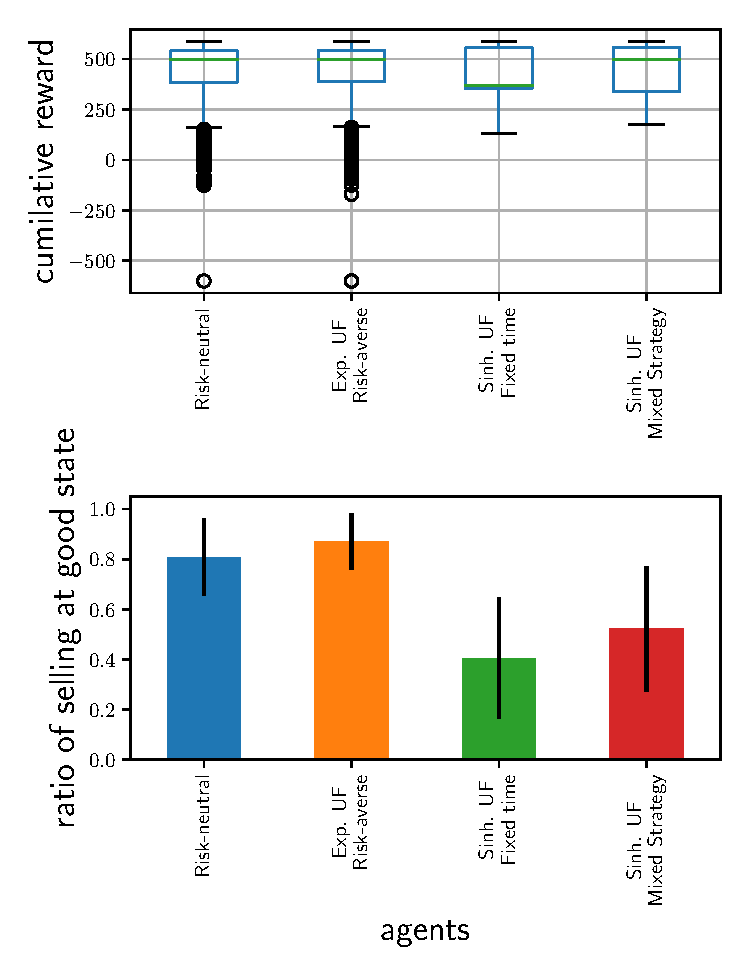
\includegraphics[width=0.8\linewidth]{img/performance.pdf}
    \caption{Average reward and ratio of selling in the good state.}
\end{figure}
